%% Introduction
%%=========================================

\chapter{Introduction}
The Oxford English Dictionary defines ``digitization" as the action or process of digitizing. Digitizing means the conversation of analogue data into digital form \cite{misc-oed-digitization}. As the world grows more and more digital, the need to digitize increases proportioned. Digitizing data makes the data easier to preserve, access, and share.

There exists countless projects to digitize books, records, and historical documents. In 2009, the National Library of Norway launched Bokhylla.no (The bookshelf). Bokhylla.no is a project to provide online access to literature published in Norwegian. The service will contain about 250 000 books when it is completed in 2017 \cite{misc-nb-digial-library}.

While simply scanning the books will suffice to make the literature available online, other technologies are needed to actually index the content. By indexing, we mean the process of capturing the scanned text and converting it into editable and searchable data. With indexed data, the actual content is available to use. This makes the data more accessible, and opens new ways of presenting the data. Indexed data makes it for example possible to perform full text search, and can also be used to give increased accessibility to blind and visually impaired users via text-to-speech technologies.

\section{Optical character recognition}
\red{This section needs some cleaning. Remove subsection? Write into one?}
While a scanner identifies the ink on the paper, it does not know, or care, which characters or symbols the ink is representing. In order to make sense of the scanned content, we use use optical character recognition, or OCR for short. OCR is the task of identifying printed characters and symbols using computer software. We can use OCR to index the entire content of the book, making it searchable.

\subsection{History and previous research}
In 1929 G. Tauschek obtained a patent in Germany on OCR that he called a ``Reading machine" \cite{misc-patent-tauschek}. In 1933 P. W. Handel did the same in the US with what he called a ``Statistical machine" \cite{misc-patent-handel}. These two patents are the first machines that could recognize characters written printed on a paper. The ``Reading machine" patent described it as an improved form of scanning device that used light rays and a light sensitive device to compare and match pictures, representations or other objects \cite{misc-tauschek1935reading}. This approach is known as a ``template matching method" \cite{article-mori1992historical}. 

The next big leap in OCR came with the commercial computer. \red{More about the development of OCR.}

\red{More about research today on OCR.}

\section{Context}
OCR is an incredible broad area. An astounding amount of research, approaches and technological solutions are already written and developed. Researching the field of OCR further would require to find something new to investigate. The idea of using character signatures came from extensive study of previous work in the area of OCR by the author. Doing classification this particular way has not, as far as the author could find, been done before. \red{Add some more here.}

\section{Problem definition}
The goal is to make OCR possible in a very limited search space. Our goal is to use the ``signature" of a character to classify it.

By ``signature", we mean that we take characters and only use a horizontal line with a low height to classify it. In \ref{fig:thesis-signature} we have the word ``THESIS". The original characters have a height of 50 pixels, but to do our classification, we only use one pixel of the total height of the characters. The line that defines the signature for this word is highlighted in the figure for illustration purposes.

\begin{figure}[ht]
    \centering
    \includegraphics[width=0.7\textwidth]{fig/chapter1/signature.png}
    \caption{Illustration of a word with a signature with a height of one pixel}
    \label{fig:thesis-signature}
\end{figure}

\red{Do we need this here?} The illustration in \ref{fig:thesis-signature} uses the sans-serif font Arial \cite{misc-arial-font}. As a \gls{sans-serif} font, the letters are clean, with no \gls{serif}s present. A few things are worth pointing out from the illustration to emphasise potential challenges with classifying via signatures.

\begin{itemize}
    \item The stroke from the T and the I are the same width, which makes them indistinguishable from each other.
    \item Because Arial is not monospaced, the spacing between each letter vary, depending on the letter before and their individual width.
\end{itemize}

\subsection{Example of use}
Markus ``Notch" Persson is a Swedish video game programmer and designer. He is most famous for crating the highly praised game Minecraft. During development of the game, Persson was a inveterate user of Twitter, and used to hint or tease upcoming features of the game. On June 12th 2011, Persson Tweeted the following Tweet:

\begin{figure}[ht]
    \centering
    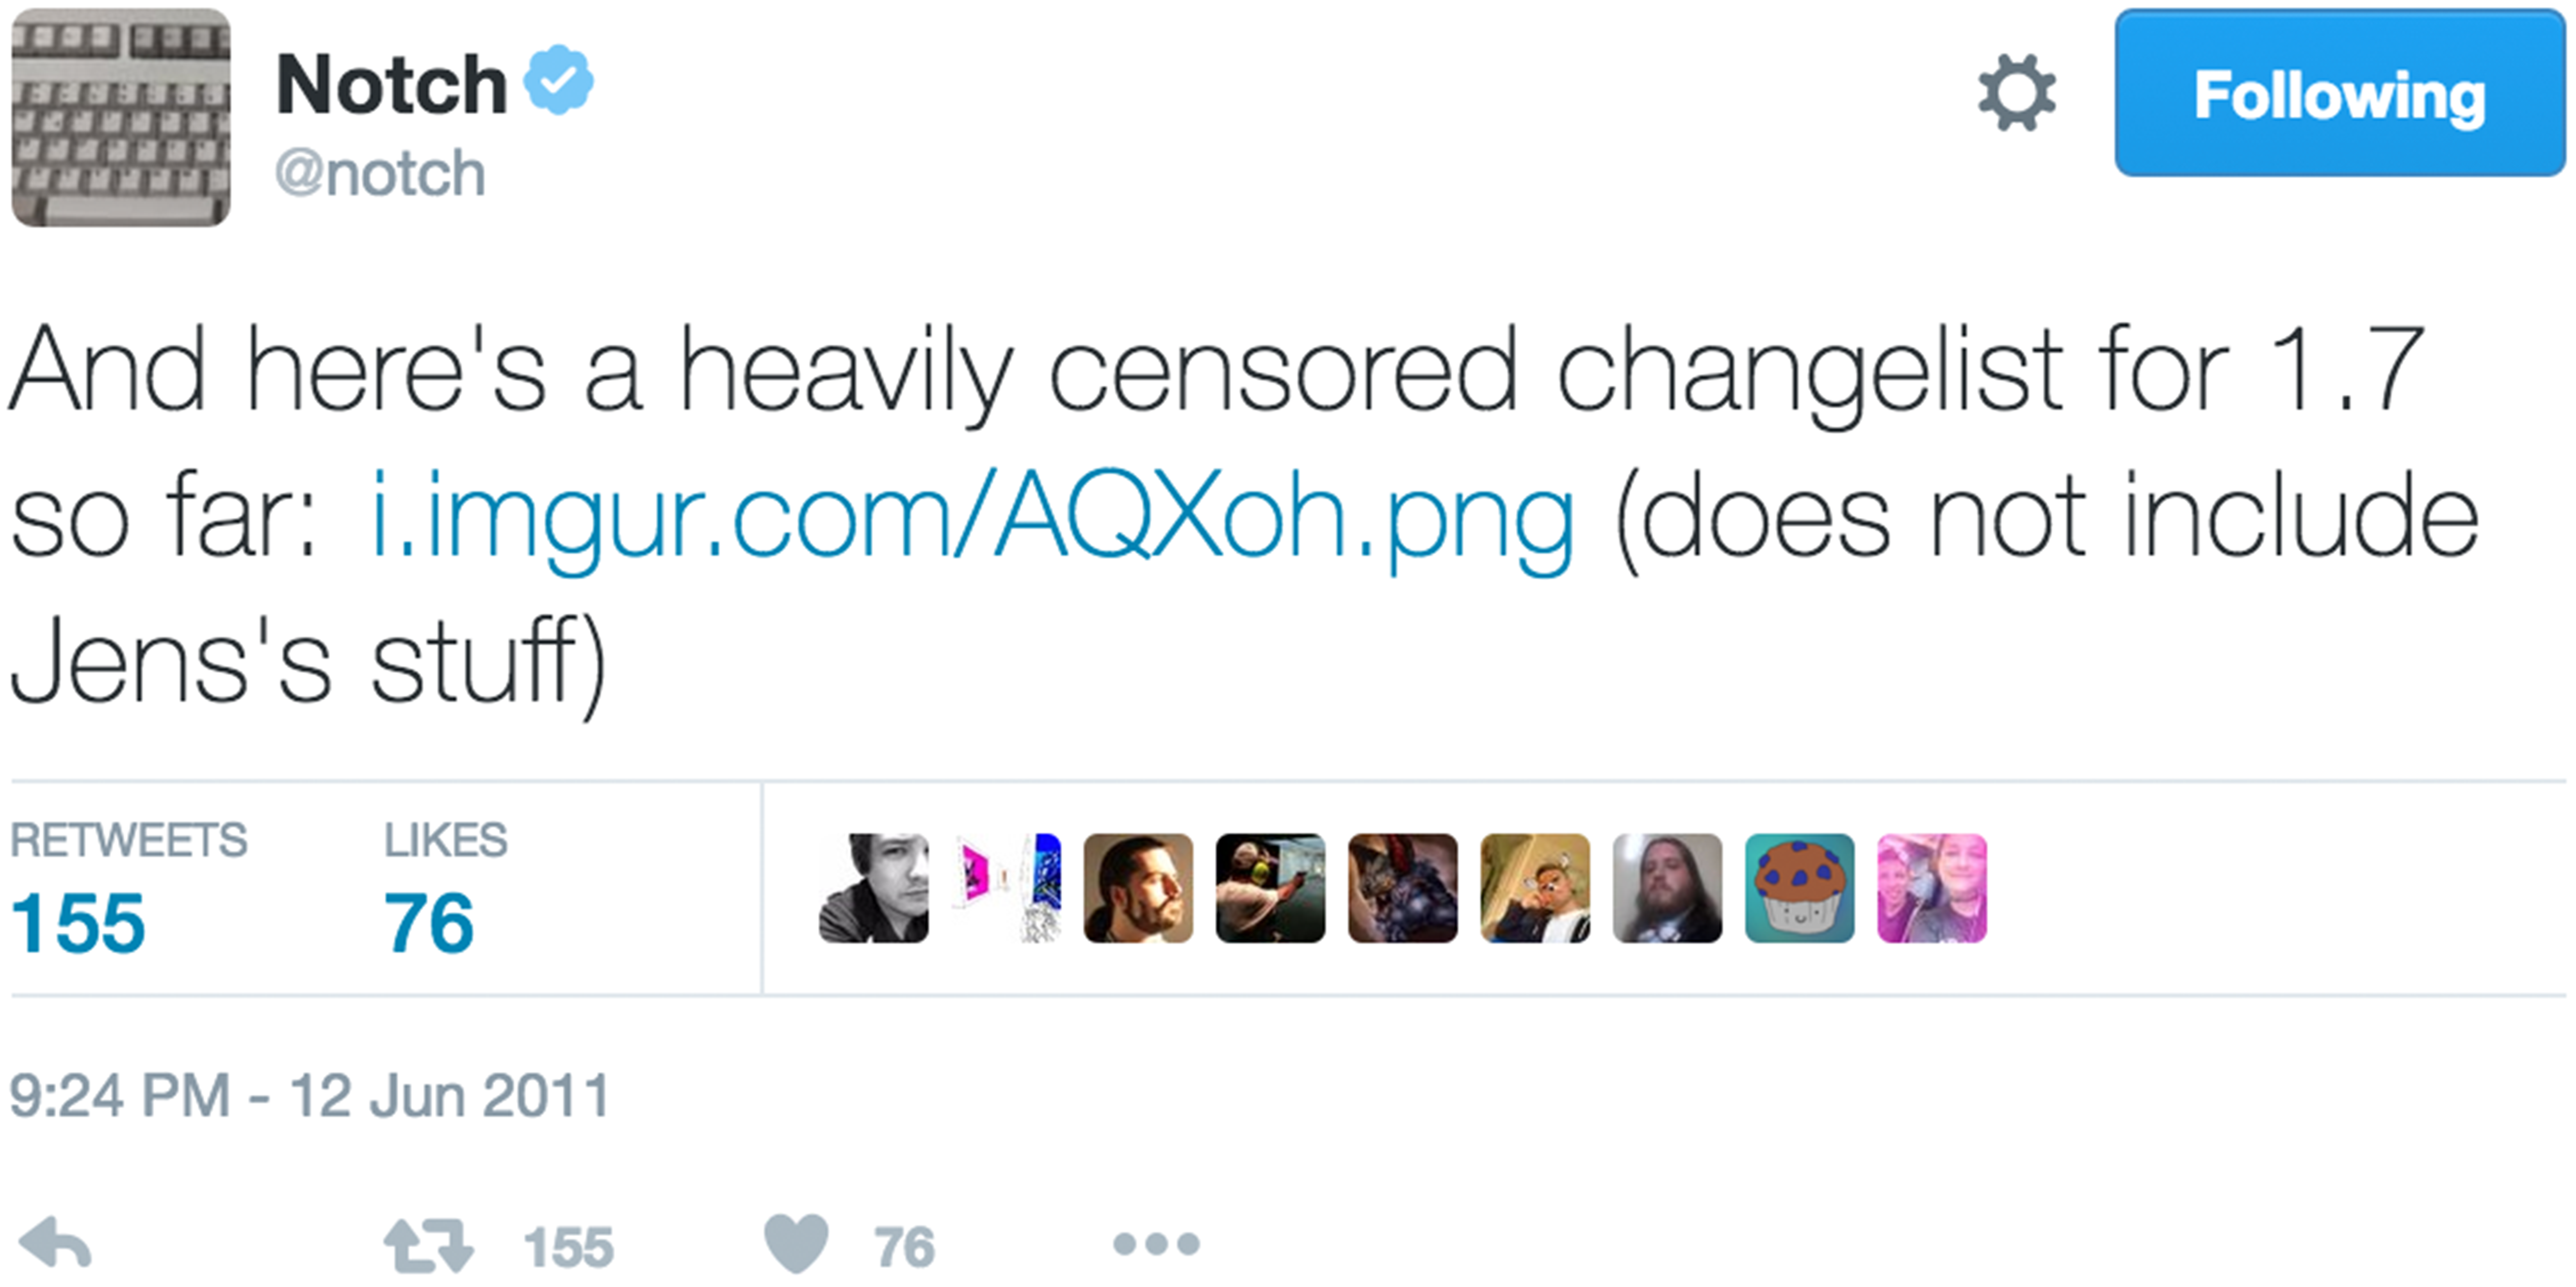
\includegraphics[width=0.7\textwidth]{fig/chapter1/notch_tweet.png}
    \caption{Print screen of Tweet from notch\protect\footnotemark}
\end{figure}
\footnotetext{Tweet and image used with the consent of Markus Persson. \href{https://twitter.com/notch/status/790531003169341440}{
    \nolinkurl{https://twitter.com/notch/}\\\nolinkurl{status/790531003169341440}}
}

The image he is referring to looks like this:

\begin{figure}[ht]
    \centering
    \includegraphics[width=0.7\textwidth]{fig/chapter1/notch_eclipse.png}
    \caption{Blurred image of Minecraft 1.7 changelog from @notch's Tweet}
\end{figure}

The image looks like it is taken inside a text editor or \gls{IDE}. There is a file currently opened, with several other files, or tabs, partially visible at the top of the image. The file that is currently opened seems to be a changelog for the upcoming 1.7 version of Minecraft, with the new major version written on the first line, followed by a list of changed. The content is mostly burred out, showing only parts of the first letter on each line and the content of some longer lines. The image is also cropped so that the file names for the files that are currently opened in the project is not displayed.


\red{Perhaps add some more here?}

\section{Personal motivation}
As the problem to solve was proposed by the author himself, it was naturally something he felt was interesting to research. He had previously played with OCR in various artificial intelligence courses at the university. Working with neural networks and Bayes Models were some of the highlights from these courses, technologies that hopefully could be used to do signature classification. \red{Add some more here.}

\section{Goals}
\red{TODO}

\section{Structure of thesis}
\red{TODO}